% Document settings
\documentclass[a4paper,11pt]{article}

% Packages
  % math formulas
\usepackage{amsmath,amsthm,amssymb}
  % graphics
\usepackage{graphicx}
\usepackage{wrapfig}
  % plots
\usepackage{pgfplots}
  % other
\usepackage[warn]{mathtext}
\usepackage{cmap}
\usepackage[T1,T2A]{fontenc}
\usepackage[utf8]{inputenc}
\usepackage[english,russian]{babel}

% Package settings
%% graphicx
\graphicspath{{Pictures/}}
\DeclareGraphicsExtensions{.pdf,.png,.jpg}
%% pgfplots
\pgfplotsset{width=10cm,compat=1.9}

% Title
\title{Отчет о выполнении работы №1.4.1\\Изучение экспериментальных погрешностей на примере физического маятника}
\author{Воейко Андрей Александрович, Б01-109}
\date{Долгопрудный, 2021}

% Document
\begin{document}
\maketitle
\newpage
\section{Аннотация.}
В работе проверяется справедливость формулы для периода колебаний физического маятника, теоремы Гюйгенса, определяется ускорение свободного падения.
\section{Теоретические сведения.}
На рисунке~\ref{fig:img1} изображен стрежень без груза. Момент инерции относительно точки подвеса вычисляется по формуле~\ref{eq1}.
\begin{wrapfigure}{r}{0.3\textwidth}
  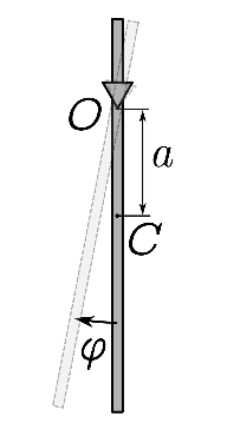
\includegraphics[scale = 0.75]{pic1.png}
  \caption{Стержень в качнестве физического маятника.}
  \label{fig:img1}
\end{wrapfigure}
\begin{equation}    \label{eq1}
  I_{0} = \frac{m_{0}l^{2}}{12} + m_{0}a^{2},
\end{equation}
где $I$ -- момент инерции, $l$ -- длина стержня, $m_{0}$ -- масса стержня с призмой, $a$ -- расстояние от точки подвеса до центра масс.\newline
Возвращающрий момент силы тяжести равен:
\begin{equation}    \label{eq2}
  M = -m_{0}g a \sin{\phi} \approx -m_{0}g a \phi.
\end{equation}
Таким образом,
$$\frac{d^{2}\phi}{dt^{2}} \sim - \phi.$$
Период цолебаний можно найти по формуле~\ref{eq3}.
\begin{equation}    \label{eq3}
  T = 2 \pi \sqrt{\frac{I}{m_{0}ga}\ } = 2 \pi \sqrt{\frac{\frac{l^{2}}{12} + a^{2}}{ga}\ }
\end{equation}
Приведенная длина физического маятника $l_{пр}$ (взята из $T = 2 \pi \sqrt{\frac{l}{g}\ }$):
\begin{equation}    \label{eq4}
  l_{пр} = a + \frac{l^{2}}{12a}.
\end{equation}
Рсстояние дто груза до центра масс $x_{ц}$:
\begin{equation}    \label{eq5}
  x_{ц} = \frac{m_{0}a + m_{г}y}{m_{0} + m_{г}},
\end{equation}
где $m_{0}$ -- масса стержня с призмой, $a$ -- расстояние от центра масс без груза до призмы, $m_{г}$ -- масса груза, $y$ -- расстояние от призмы до ц. м. груза.\newline
Поскольку груз имеет сложную форму, следует один раз вычислить $x_{ц}$ для первого измерения, а потом находить ее изменение по изменению $y$ из формулы~\ref{eq5}. Тогд апериод колебаний составит:
\begin{equation}    \label{eq6}
  T = 2 \pi \sqrt{\frac{I_{0} + m_{г} y^{2}}{(m_{0} + m_{г}) g x_{ц}}\ }.
\end{equation}
Отсюда вывводим $g$:
\begin{equation}    \label{eq7}
  g = \frac{I_{0} + m_{г}y^{2}}{(m_{0} + m_{г}) x_{ц}} \cdot \frac{4 \pi^{2}}{T^{2}} = \frac{4 \pi^{2}}{T^{2}} \cdot \frac{m_{0}(\frac{l^{2}}{12} + a^{2}) + m_{г} y^{2}}{m_{0}a + m_{г}y}.
\end{equation}
\section{Оборудование и экспериментальная установка.}
\subsection{Используемое оборудывние и погрешности его использования.}
В работе используются:
\begin{itemize}
        \item Штангенциркуль. Погрешность -- $\pm 0,01\ см$.
        \item Линейка. Погрешность -- $\pm 0,1\ см$.
        \item Счетчик. Погрешность -- $\pm 0,01\ с$.
        \item Весы. Погрешность -- $\pm 0,1\ с$.
        \item Металлический стержень.
        \item Дополнительный груз.
        \item Подставка с отсрой гранью для определения центра масс стержня.
\end{itemize}
\subsection{Вес и длина объектов.}
Измерим массу стержня, призмы и груза. Также измерим длины этих объектов и расстояние от верхнего конца стрежня до центра масс с призмой и без, а также расстояние от цетнра масс до точки подвеса (до нижнего края призмы). Результаты занесем в таблицу~\ref{table:tab1}.
% Табл. 1 {{{
\begin{table}[h!]
\centering
\begin{tabular}{ ||l|c|| }
  \hline
  Величина & Значение \\
  \hline
  Масса стержня $m_{ст}$, $г$ & $869,8 \pm 0,1$ \\
  \hline
  Масса призмы $m_{п}$, $г$ & $74,9 \pm 0,1$ \\
  \hline
  Масса стержня & $944,7 \pm 0,2$ \\
  с призмой $m_{0}$, $г$ & \\
  \hline
  Масса груза $m_{г}$, $г$ & $376,2 \pm 0,1$ \\
  \hline
  Длина стрежня $l$, $см$ & $100,1 \pm 0,1$ \\
  \hline
  Расстояние от центра & \\
  масс до верхнего & $50,0 \pm 0,1$ \\
  конца без призмы, $см$ & \\
  \hline
  Расстояние от центра & \\
  масс до верхнего & $47,6 \pm 0,1$ \\
  конца с призмой, $см$ & \\
  \hline
  Расстояние от & \\
  центра масс & $25,7 \pm 0,1$ \\
  до призмы $a$, $см$ & \\
  \hline
\end{tabular}
    \caption{Массы и длины исследуемых объектов.}
    \label{table:tab1}
\end{table}\newline
% }}}
\section{Результаты измерений и обработка данных.}
\subsection{Результаты измерений.}
\subsubsection{Предварительные измерения периода колебаний.} %%%%% Предварительные %%%%%
Проведем предварительные измерения периода колебаний. Для этого измерим время 20 колебаний, а затем поделим полученное значение на 20.\newline
$t_{предв} = 29,2 \pm 0,6\ с$. Повторные измерения дали идентичный результат.\newline
$T_{предв} = 1,46 \pm 0,03\ с$\newline
$y = 46,6\ см$\newline
По формуле~\ref{eq7} найдем $g$:
$$g = \frac{4 \cdot 3,14^{2}}{1,46^{2}} \cdot \frac{944,7 \cdot (\frac{1,001^{2}}{12} + 0,257^{2}) + 376,2 \cdot 0,466^{2}}{944,7 \cdot 0,257 + 376,2 \cdot 0,466} = 9,84 \pm 0,01\ \frac{м}{с^{2}}.$$
\subsubsection{Измерение периода колебаний.} %%%%% Период и g %%%%%
Проведем еще 9 измерений. Результаты всех измерений, включая и предварительные, занесем в таблицу~\ref{table:tab2}.
% Табл. 2 {{{
\begin{table}[h!]
\centering
\begin{tabular}{ ||c|c|c|c|c|c|c|| }
  \hline
  № & $y$, $см$ & $x_{ц}$, $см$ & $n$ & $t$, $с$ & $T$, $с$ & $g$, $\frac{м}{с^{2}}$ \\
  \hline
  $1$ & $46,4 \pm 0,1$ & $31,7 \pm 0,1$ & $20$ & $29,2 \pm 0,6$ & $1,462$ & $9,84 \pm 0,06$ \\
  $2$ & $50,9 \pm 0,1$ & $32,9 \pm 0,1$ & $20$ & $29,7 \pm 0,6$ & $1,488$ & $9,802 \pm 0,06$ \\
  $3$ & $55,9 \pm 0,1$ & $34,3 \pm 0,1$ & $20$ & $30,3 \pm 0,6$ & $1,517$ & $9,80 \pm 0,06$ \\
  $4$ & $58,9 \pm 0,1$ & $35,1 \pm 0,1$ & $20$ & $30,7 \pm 0,6$ & $1,534$ & $9,814 \pm 0,06$ \\
  $5$ & $60,9 \pm 0,1$ & $35,7 \pm 0,1$ & $20$ & $30,9 \pm 0,6$ & $1,547$ & $9,811 \pm 0,06$ \\
  $6$ & $57,3 \pm 0,1$ & $34,7 \pm 0,1$ & $20$ & $30,5 \pm 0,6$ & $1,525$ & $9,808 \pm 0,06$ \\
  $7$ & $54,3 \pm 0,1$ & $33,9 \pm 0,1$ & $20$ & $30,1 \pm 0,6$ & $1,507$ & $9,807 \pm 0,06$ \\
  $8$ & $51,3 \pm 0,1$ & $33,0 \pm 0,1$ & $20$ & $29,8 \pm 0,6$ & $1,490$ & $9,799 \pm 0,06$ \\
  $9$ & $48,3 \pm 0,1$ & $32,1 \pm 0,1$ & $20$ & $29,4 \pm 0,6$ & $1,473$ & $9,811 \pm 0,06$ \\
  $10$ & $46,3 \pm 0,1$ & $31,6 \pm 0,1$ & $20$ & $29,3 \pm 0,6$ & $1,462$ & $9,803 \pm 0,06$ \\
  \hline
\end{tabular}
    \caption{Массы и длины исследуемых объектов.}
    \label{table:tab2}
\end{table}\newline
% }}}
Среднее значение ускорение свободного падения составило $\overline{g} = 9,809\ \frac{м}{с^{2}}$.\newline
Стандартная ошибка среднего -- $\sigma_{\overline{g}} = 0,004\ \frac{м}{с^{2}}$.\newline
Таким образом, ускорение свободного падения равняется $g = 9,809 \pm 0,004\ \frac{м}{с^{2}}$.
\subsection{Обработка данных.}
\subsubsection{Зависимость периода колебаний от положения груза.}
Построим график зависимости периода колебаний $T$ от положения груза $y$. График представлен на рисунке~2.
\begin{center}
\begin{tikzpicture}
\begin{axis}[
	xlabel = {$y$},
	ylabel = {$T$},
    grid = major,
	minor tick num = 2
]
\addplot[
    blue,
    mark size = 1.5 pt,
    only marks,
]
table {
	x    y
  46.4 1.462
  50.9 1.488
  55.9 1.517
  58.9 1.534
  60.9 1.547
  57.3 1.525
  54.3 1.507
  51.3 1.490
  48.3 1.473
  46.3 1.462
};
\end{axis}
\end{tikzpicture}\newline
Рис. 2: График зависимоти периода колебаний $T$ от положения груза $y$.\newline
\end{center}
\subsubsection{Зависимость периода колебаний от положения груза.}
Построим график зависимости величины $T^{2}x_{ц}$ от величины $y^{2}$. График представлен на рисунке~3. Аппроксимируем прямую к прямой $(T^{2}x_{ц}) = a + b(y^{2})$. Заметим, согласно формуле~\ref{eq6} $a = \frac{4\pi^{2} I_{0}}{(m_{0} + m_{г})g}$, а $b = \frac{4\pi^{2}m_{г}}{(m_{0} + m_{г})g}$.\newline
Итак, $b = \frac{\left<xy\right> - \left<x\right>\left<y\right>}{\left<x^{2}\right> - \left<x\right>^{2}} = \frac{0,2175 - 0,2143}{0,08326 - 0,08043} = \frac{32}{28,3} = 1,1307$.\newline
$\sigma_{b} \approx \frac{1}{\sqrt{n}}\sqrt{\frac{\left<y^{2}\right> - \left<y\right>^{2}}{\left<x^{2}\right> - \left<x\right>^{2}} - b^{2}\ } = 0,025$.\newline
Отсюда $g = 9,95 \pm 0,23\ \frac{м}{с^{2}}$.\newline
$a = \left<y\right> - b\left<x\right> = 0,7556 - 0,3207 = 0,435$.\newline
$\sigma_{a} = \sigma_{b}\sqrt{\left<x^{2}\right> - \left<x\right>^{2}\ } = 0,001$.
\begin{center}
\begin{tikzpicture}
\begin{axis}[
	xlabel = {$y^{2}$},
	ylabel = {$T^{2}x_{ц}$},
    xmin = 0.2,
    xmax = 0.4,
    ymin = 0.662,
    ymax = 0.8874,
    grid = major,
	minor tick num = 6
]
\addplot[
    blue,
    mark size = 2 pt,
    only marks,
]
table {
	x     y
  0.215 0.678
  0.259 0.728
  0.312 0.789
  0.347 0.826
  0.371 0.854
  0.328 0.807
  0.295 0.770
  0.263 0.733
  0.233 0.696
  0.214 0.675
};
\addplot[
    blue,
    no marks,
    % yes Marx
]
table {
	x    y
	0.2  0.661
  0.4  0.8873
};
\end{axis}
\end{tikzpicture}\newline
Рис. 3: График зависимоти величины $T^{2}x_{ц}$ от величины $y^{2}$.\newline
\end{center}
\section{Выводы.}
В ходе работы было вычилено значение $g$ двумя различными спопобами -- методом подсчета для каждого измерения с вычислением среденего и методом аппроксимации к прямой графика $T^{2}x_{ц}$ от $y^{2}$ с нахождением коэффицентов. Первый способ, как и ожидалось, показал большую точность, но для обоих способов реальное табличное значение $g$ лежит в пределах погрешности.
\end{document}
